\question \textbf{Measures with multiple thresholds}
  
Create multiple confusion matrices by considering all possible threshold values. Assume that the test data set contains two positives and two negatives. The table below shows the scores given by a model that gives higher scores for the alignments with higher similarities. 

\begin{table}[H]
\centering
\begin{tabular}{|l|l|l|l|l|}
\hline
Test set label & P   & P   & N   & N   \\ \hline
Model score    & 2.1 & 3.1 & 2.3 & 1.2 \\ \hline
\end{tabular}
\end{table}

\vspace{0.1 in}

\begin{parts}

%% (a)
  \part Fill the labels that match the sorted scores

\begin{table}[H]
\centering
\begin{tabular}{|l|l|l|l|l|}
\hline
Test set label &    &     &     &    \\ \hline
Model score    & 2.1 & 3.1 & 2.3 & 1.2 \\ \hline
\end{tabular}
\end{table}

%% (b)
\part Fill the labels predicted by different threshold values.

\begin{figure}[H]
      \centering
      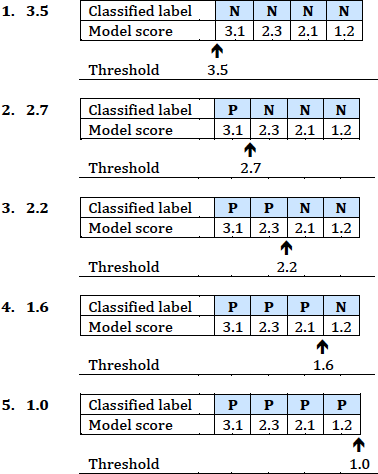
\includegraphics[width=0.6 \textwidth]{fig07/thresholds_solution.png}
\end{figure}

%
% NEWPAGE
%
\newpage

%% (c)
  \part Use the labels in (a) and (b) and calculate TP, FP, TN, and FN for all threshold values.

\begin{table}[H]
\centering
\begin{tabular}{|l|c|c|c|c|}
\hline
Threshold & \multicolumn{1}{l|}{TP}   & \multicolumn{1}{l|}{FP}   & \multicolumn{1}{l|}{TN}   & \multicolumn{1}{l|}{FN}   \\ \hline
3.5       & \cellcolor[HTML]{CCE5FF}0 & \cellcolor[HTML]{CCE5FF}0 & \cellcolor[HTML]{CCE5FF}2 & \cellcolor[HTML]{CCE5FF}2 \\ \hline
2.7       & \cellcolor[HTML]{CCE5FF}1 & \cellcolor[HTML]{CCE5FF}0 & \cellcolor[HTML]{CCE5FF}2 & \cellcolor[HTML]{CCE5FF}1 \\ \hline
2.2       & \cellcolor[HTML]{CCE5FF}1 & \cellcolor[HTML]{CCE5FF}1 & \cellcolor[HTML]{CCE5FF}1 & \cellcolor[HTML]{CCE5FF}1 \\ \hline
1.6       & \cellcolor[HTML]{CCE5FF}2 & \cellcolor[HTML]{CCE5FF}1 & \cellcolor[HTML]{CCE5FF}1 & \cellcolor[HTML]{CCE5FF}0 \\ \hline
1         & \cellcolor[HTML]{CCE5FF}2 & \cellcolor[HTML]{CCE5FF}2 & \cellcolor[HTML]{CCE5FF}0 & \cellcolor[HTML]{CCE5FF}0 \\ \hline
\end{tabular}
\end{table}

%% (d)
  \part Use the result in (c) and calculate basic evaluation measures. Round off the answer to one decimal place if necessary.

\begin{table}[H]
\centering
\begin{tabular}{|l|c|c|c|}
\hline
Threshold & \multicolumn{1}{l|}{Specificity} & \multicolumn{1}{l|}{1 - specificity} & \multicolumn{1}{l|}{Sensitivity} \\ \hline
3.5       & \cellcolor[HTML]{CCE5FF}1        & \cellcolor[HTML]{CCE5FF}0            & \cellcolor[HTML]{CCE5FF}0        \\ \hline
2.7       & \cellcolor[HTML]{CCE5FF}0.5      & \cellcolor[HTML]{CCE5FF}0.5          & \cellcolor[HTML]{CCE5FF}0.5      \\ \hline
2.2       & \cellcolor[HTML]{CCE5FF}0.5      & \cellcolor[HTML]{CCE5FF}0.5          & \cellcolor[HTML]{CCE5FF}0.5      \\ \hline
1.6       & \cellcolor[HTML]{CCE5FF}0        & \cellcolor[HTML]{CCE5FF}1            & \cellcolor[HTML]{CCE5FF}1        \\ \hline
1         & \cellcolor[HTML]{CCE5FF}0        & \cellcolor[HTML]{CCE5FF}1            & \cellcolor[HTML]{CCE5FF}1        \\ \hline
\end{tabular}
\end{table}

%% (e)
  \part Draw a ROC curve for the calculated evaluation measures in (d).

\begin{figure}[H]
      \centering
      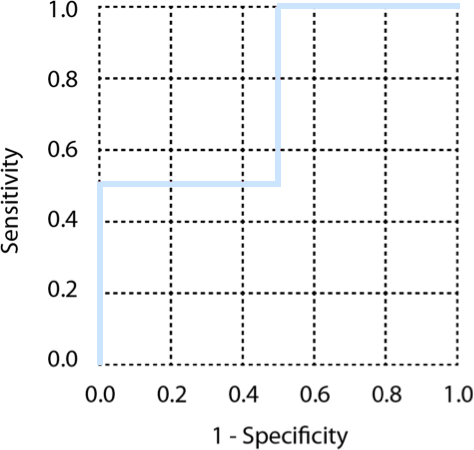
\includegraphics[width=0.3 \textwidth]{fig07/roc_sol.png}
\end{figure}

%% (f)
  \part Calculate the area under the curve of the curve in (e).
  
\begin{solution}[0.35 in]
0.75
\end{solution}

%% (g)
  \part Evaluate the ROC curve in your own words.
  
\begin{solution}[0.35 in]
The model performs better than random classifiers
\end{solution}

\end{parts}

